\documentclass[conference]{IEEEtran}
\IEEEoverridecommandlockouts
% The preceding line is only needed to identify funding in the first footnote. If that is unneeded, please comment it out.
\usepackage{cite}
\usepackage{amsmath,amssymb,amsfonts}
\usepackage{algorithmic}
\usepackage{graphicx}
\usepackage{textcomp}
\usepackage{xcolor}
\def\BibTeX{{\rm B\kern-.05em{\sc i\kern-.025em b}\kern-.08em
    T\kern-.1667em\lower.7ex\hbox{E}\kern-.125emX}}
\begin{document}

\title{Real-Time Monitoring and Remote Guidance of\\ Mobile Robots Using Multimodal Digital Twins}

\author{\IEEEauthorblockN{Trung Kien La}
\IEEEauthorblockA{\textit{Dept. of Comp. Science \& Engineering} \\
\textit{Frankfurt University of Applied Sciences}\\
Frankfurt a.M., Germany \\
trung.la@stud.fra-uas.de}
\and
\IEEEauthorblockN{René Harmann}
\IEEEauthorblockA{\textit{Dept. of Comp. Science \& Engineering} \\
\textit{Frankfurt University of Applied Sciences}\\
Frankfurt a.M., Germany\\
rene.harmann@fb2.fra-uas.de}
\and
\IEEEauthorblockN{Eric Guiffo Kaigom}
\IEEEauthorblockA{\textit{Dept. of Comp. Science \& Engineering} \\
\textit{Frankfurt University of Applied Sciences}\\
Frankfurt a.M., Germany \\
kaigom@fb2.fra-uas.de}

}

\maketitle

\begin{abstract}
    Although digital twins have been playing a pivotal
    role in the management of the lifecycle of physical robotic
    systems of systems, they have hardly been employed to guide
    mobile robots in real-time. In fact, the guidance of such systems
    requires functionalities, including the perception of targeted
    locations and avoidance of collisions, that build upon spatial
    information beyond internal robot states usually acquired using
    proprioceptive sensors. In this case, exteroceptive sensors help
    meet this demand. Nevertheless, such sensors have received little
    attention thus far in the development of digital twins. On the
    other hand, the completion of various spatial objectives, such as
    reverse motions, might require the awareness of the historical
    internal state of the distant robot. For instance, the current
    energy budget is likely to constrain the reachability of the
    initial state after a while, even when spatially and kinematically
    feasible. We therefore embrace these challenges with a multi-
    modal approach to provide and employ digital twin of mobile
    robots. We collect data about the internal state and camera-
    captured neighborhood of the robot in real-time. The robot
    operator is thereby provided with a multi-dimensional state and
    perception view that characterizes the robot, elevates situational
    awareness, and facilitates decision support. We then develop a
    versatile graphical interface that helps monitor and steer mobile
    robots. Since the bidirectional approach is intuitive and user
    friendly, even novices can remotely guide a mobile robot with
    multi-modal situational awareness. We show the versatility and
    effectiveness of our approach in use case scenarios in practice.
\end{abstract}

\begin{IEEEkeywords}
    Robotics, Multimodal Data, Digital Twins, In-
    dustry 4.0, Industry 5.0, Society 5.0, Human-Mobile Robot-
    Interaction, Systems of Systems
\end{IEEEkeywords}

\section{Introduction}
The Robot Operating System (ROS) is one of the most popular pieces of robot middleware when it comes to creating a basis for robots and creating robot applications \cite{rosOrg}. 
Nevertheless, it is a challenge for people with little or no knowledge of robot software to familiarize themselves with this software. 
Especially people who are dependent on the help of robots should have intuitive access to these robots.
With this in mind, a web application was developed that is as platform-independent as possible. 
This web application enables users to monitor and control the robot located in the local network. 
Furthermore, relevant data such as the battery status and the temperatures of the motors are visualised. 
The application can also be accessed by any device with web browser support.
\begin{figure}[htbp]
    \centerline{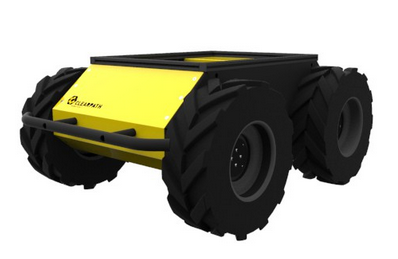
\includegraphics[width=8.9cm]{Pictures/Husky_clearpath.png}}
    \caption{Picture of the Husky UGV by Clearpath}
    \label{fig:huskyClearpath}
\end{figure} 
The robot we use is the Husky Unmanned Ground Vehicle (UGV) from Clearpath, which is a medium-sized mobile robotics platform as shown in Fig. \ref{fig:huskyClearpath}.
With a maximum payload of 75 kg, other robots, peripherals and tools, for example, can be transported or mounted on it \cite{huskyClearpath}. 




\section{State of the Art}
C. Crick et al.  

\subsection{Maintaining the Integrity of the Specifications}

The IEEEtran class file is used to format your paper and style the text. All margins, 
column widths, line spaces, and text fonts are prescribed; please do not 
alter them. You may note peculiarities. For example, the head margin
measures proportionately more than is customary. This measurement 
and others are deliberate, using specifications that anticipate your paper 
as one part of the entire proceedings, and not as an independent document. 
Please do not revise any of the current designations.

\section{Implementation and Design}
The system architecture of the web application can be divided into a backend and a frontend, whereby various tools and frameworks are used.
\subsection{Backend}
The web application is a Flask application. Flask is a micro web framework that is characterized by providing the core features to create a python web based application. 
Therefore, Flask is very flexible and also highly extensible \cite{flasksqlite}.
\begin{itemize}
\item Test
\item DDS
\item standard
\item teams
\item 
\end{itemize}

\subsection{Frontend}


\subsection{Equations}

\subsection{\LaTeX-Specific Advice}



\subsection{Some Common Mistakes}

\begin{thebibliography}{00}
\bibitem{rosOrg} “ros.org,”
2024.
[Online].
Available:
https://ros.org
\bibitem{huskyClearpath} “clearpathrobotics.com,”
2024.
[Online].
Available:
https://clearpathrobotics.com/husky-unmanned-ground-vehicle-robot/
\bibitem{rosbridgeOkState} Crick, C., Jay, G., Osentoski, S., Pitzer, B., and Jenkins, O. C. ``Rosbridge: Ros
for non-ros users,'' in Robotics Research, Springer, 2017, pp. 493--504.
\bibitem{flasksqlite} Suraya, Muhammad Sholeh, ``Designing and Implementing a Database for Thesis Data,'' in International Journal of Engineering, Science \& InformationTechnology (IJESTY)
Volume 2, No. 1, 2022, pp. 9--14, eISSN: 2775-2674


\end{thebibliography}
\vspace{12pt}
\color{red}
IEEE conference templates contain guidance text for composing and formatting conference papers. Please ensure that all template text is removed from your conference paper prior to submission to the conference. Failure to remove the template text from your paper may result in your paper not being published.

\end{document}
